\setcounter{chapter}{3}
\chapter{Software implementation}
\label{Software}
% 

\includegraphics[width=.075\textwidth]{gfx/Scihub_raven.png}
\cleanchapterquote{Journal paywalls are an example of something that works in the reverse direction, making communication less open and efficient.}{Alexandra Elbakyan}{}
% 
% \tikz[remember picture,overlay] \node[inner sep=0pt] at (0,0){
\includegraphics[height=7em]{gfx/Scihub_raven.png}};
% \hspace{-10em}

% \clearpage opacity=0.3,
% 
\comment{\paragraph{Ziele:} 
\begin{itemize}
    \item User-Friendly: Python
    \item C++ 
    \item usw.
\end{itemize}}
%
\cite{pybind11}
% 
\section{Introduction}
\ac{GM}
% 
\section{Framework}
The software package \ac{fastPLI} \cite{fastpli} is build as a \python{} \cite{Python3} package.
% 
To explain Python packages, first Python modules needs to be explained.
% 
Simply said, a Python module is a collection of executable functions.
They can however also contain other modules.
Their structure is exactly build up like a file structure. 
% 
A \python{} package on the other side is a collection of python code and modules.
Their structure are indistinguishable from modules, however they contain additional instruction for the installation process.
E.\ g. \python{} can also run compiled shared \ccpp{} functions.
A \python{} package can include the instructions to compile this functions with a suitable \ccpp{} compiler and a list of all necessary additional \ccpp{} Libraries.
\\
% 
The mathematical \dummy{} are descriebed in \cref{chap:modelling}.
The following subpackeges are explained in detail.
A complete description can be found on \url{https://github.com/3d-pli/fastpli/wiki}.
% 
\begin{lstfloat}[!t]
\lstset{style=python}
\begin{lstlisting}
import fastpli
''' __version__
'''

import fastpli.analysis
''' affine_transformation
    epa
    images
    rofl
'''

import fastpli.io
''' fiber_bundles
'''

import fastpli.model.sandbox
''' fill
    shape
'''

import fastpli.model.solver
''' class Solver
    __solver.cpython.so
    _solver.py
'''

import fastpli.objects
''' fiber
    fiber_bundle
    fiber_bundles
'''

import fastpli.simulation
''' class Simpli
    __generation.cpython.so
    __simulation.cpython.so
    _simpli.py
    optic
'''

import fastpli.tools
''' label_converter
    rotation
'''
\end{lstlisting}
\caption[Overview \fastpli{} package]{Overview \fastpli{} package with containing modules}
% 	\label{alg:simulation}
\end{lstfloat}
% 
\subsection{fastpli.analysis}
\begin{lstfloat}[!t]
\lstset{style=python}
\begin{lstlisting}
import fastpli.analysis
fastpli.analysis.affine_transformation
    # apply affine transformations to images (e.g. untilt)
fastpli.analysis.epa
    # analysis of 2d PLI images
fastpli.analysis.images
    # analysis/generation of color images (FOM, VectorImages, ...)
fastpli.analysis.rofl
    # analysis tilted PLI images
\end{lstlisting}
\caption{\code{fastpli.analysis}}
% 	\label{alg:simulation}
\end{lstfloat}
% 
\subsection{fastpli.io}
\begin{lstfloat}[!t]
\lstset{style=python}
\begin{lstlisting}
import fastpli.io
fastpli.io.fiber_bundles
    # io operations for dat-files and hdf5-files
    # for the fiber_bundles format.
\end{lstlisting}
\caption{\code{fastpli.io}}\label{alg:fastpli.io}
\end{lstfloat}
% 
\paragraph{fiber\_bundles.py} contains io routines (see \cref{alg:fastpli.io}) for reading and saving fiber\_bundles into dat-files or hdf5-files. dat-files are text files which have to following structure as in \cref{alg:dat-file}. This dataformat is used to be as exchange friendly as possible for new users. \hdf{} files on the other hand are a binary dataformat \cite{hdf5}, where the individual datasets are arange in datacontainers, like the file explorer (see \cref{alg:hdf5}). The data contains 4d arrays, which are explained in \cref{sec:nerve_fiber_representation}.
% 
\begin{lstfloat}[!t]
\lstset{style=common,morecomment=[l][\color{syntax_green}]{<-},}
\begin{lstlisting}
-6.55 -18.93 -64.98 3.75 <- x y z r
-5.73 -14.89 -63.37 3.4
-4.42 -13.66 -58.95 3.05
    <- empty line indicates new fiber
-1.96 -10.07 -52.5 2.92
-1.03 -9.4 -48.62 2.93

    <- two empty lines indicates new fiber bundle
3.4 -4.02 -44.76 3.11
6.22 -1.04 -42.45 3.26
\end{lstlisting}
\caption{exemplary dat-file format. Commets are currently not allowed and are only for the readers eyes.}\label{alg:dat-file}
\end{lstfloat}
% 
\begin{lstfloat}[!t]
\lstset{style=common}
\begin{lstlisting}
GROUP "/" { # fiber_bundles path
  GROUP "0" { # id of fiber_bundle
      DATASET "0" { # id of fiber
         DATATYPE  H5T_IEEE_F64LE
         DATASPACE  SIMPLE { ( 3, 4 ) / ( 3, 4 ) }
         DATA {
         (0,0): -6.55, -18.93, -64.98, 3.75,
         (1,0): -5.73, -14.89, -63.37, 3.4,
         (2,0): -4.42, -13.66, -58.95, 3.05,
         }
      }
      DATASET "1" { # id of fiber
         DATATYPE  H5T_IEEE_F64LE
         DATASPACE  SIMPLE { ( 2, 4 ) / ( 2, 4 ) }
         DATA {
         (3,0): -1.96, -10.07, -52.5, 2.92,
         (4,0): -1.03, -9.4, -48.62, 2.93,
         }
      }
  }
  GROUP "1" { # id of fiber_bundle
      DATASET "0" { # id of fiber
         DATATYPE  H5T_IEEE_F64LE
         DATASPACE  SIMPLE { ( 2, 4 ) / ( 2, 4 ) }
         DATA {
         (0,0): 3.4, -4.02, -44.76, 3.11,
         (1,0): 6.22, -1.04, -42.45, 3.26,
         }
      }
  }
}
\end{lstlisting}
\caption{exemplary hdf5-file format.} \label{alg:hdf5}
\end{lstfloat}
% 
% 
\subsection{fastpli.model.sandbox}
\begin{lstfloat}[!t]
\lstset{style=python}
\begin{lstlisting}
import fastpli.model.sandbox
fastpli.model.sandbox.fill
    # filling of trajectaries with seed points as fiber_bundles
fastpli.model.sandbox.build
    # building of geometries
\end{lstlisting}
\caption{\code{fastpli.model.sandbox}}
% 	\label{alg:simulation}
\end{lstfloat}
% 
\subsection{fastpli.model.solver}
\begin{lstfloat}[!t]
\lstset{style=python}
\begin{lstlisting}
import fastpli.model.solver
fastpli.model.solver.Solver
    # Class wrapper for C++ class.
    # Solves any 3d configurations of fibers to a non colliding ...
\end{lstlisting}
\caption{\code{fastpli.model.solver}}
% 	\label{alg:simulation}
\end{lstfloat}
% 
\subsection{fastpli.simulation}
\begin{lstfloat}[!t]
\lstset{style=python}
\begin{lstlisting}
import fastpli.simulation
fastpli.simulation.Simpli
    # Class wrapper for C++ class.
    # Generatoes:
    #   - discretisied Tissue Volume
    #   - 3D PLI images
    #   - analysis of resultss
\end{lstlisting}
\caption{\code{fastpli.simulation}}
% 	\label{alg:simulation}
\end{lstfloat}
% 
\subsection{fastpli.tools}
\begin{lstfloat}[!t]
\lstset{style=python}
\begin{lstlisting}
import fastpli.tools
fastpli.tools.label_converter
    # conversion of discretisied tissue to 
    # maxwell-solver input format
fastpli.tools.rotation
    # rotation matricies for 3d rotaions
\end{lstlisting}
\caption{\code{fastpli.tools}}
% 	\label{alg:simulation}
\end{lstfloat}
% 
\subsection{Dependencies}
% 
\paragraph{Python:}
\begin{description}
\item[numpy:] Base N-dimensional array package \cite{2019arXiv190710121V}\\
\url{https://numpy.org/}
\item[scipy:] Fundamental library for scientific computing \cite{2019arXiv190710121V}\\
\url{https://www.scipy.org/} 
\item[numba:] Acceleration of Python Functions \cite{Lam2015}\\
\url{https://numba.pydata.org/}
\item[mpi4py:] MPI for Python \cite{Dalcn2005, Dalcn2008, Dalcin2011}\\
\url{https://bitbucket.org/mpi4py/mpi4py/src/master/}
\item[h5py:] HDF5 for Python \cite{collette_python_hdf5_2014, hdf5}\\
\url{https://www.h5py.org/}
\end{description}
% 
\paragraph{C++:}
\begin{description}
\item[MPI:] Message Passing Interface \cite{message2015mpi}\\
\url{https://www.mpi-forum.org/}
\item[OpenMP:] Open Multi-Processing, API for multi-platform shared memory multiprocessing programming \cite{dagum1998openmp}\\
\url{https://www.openmp.org/}
\item[OpenGL:] Open Graphics Library \cite{khronos}\\
\url{www.opengl.org}
\item[Pybind11:] Seamless operability between C++11 and Python \cite{pybind11}\\ \url{https://github.com/pybind/pybind11} 
\end{description}
% 
% 
\begin{figure}[!t]
\centering
\resizebox{0.95\textwidth}{!}{
 \inputtikz[true]{gfx/fastpli/fastpli_sim_pipeline}}
\caption{pipeline}
\label{fig:sim_pipeline}
\end{figure}
% 
\begin{figure}[!t]
    \centering
    \resizebox{\textwidth}{!}{\fbox{
    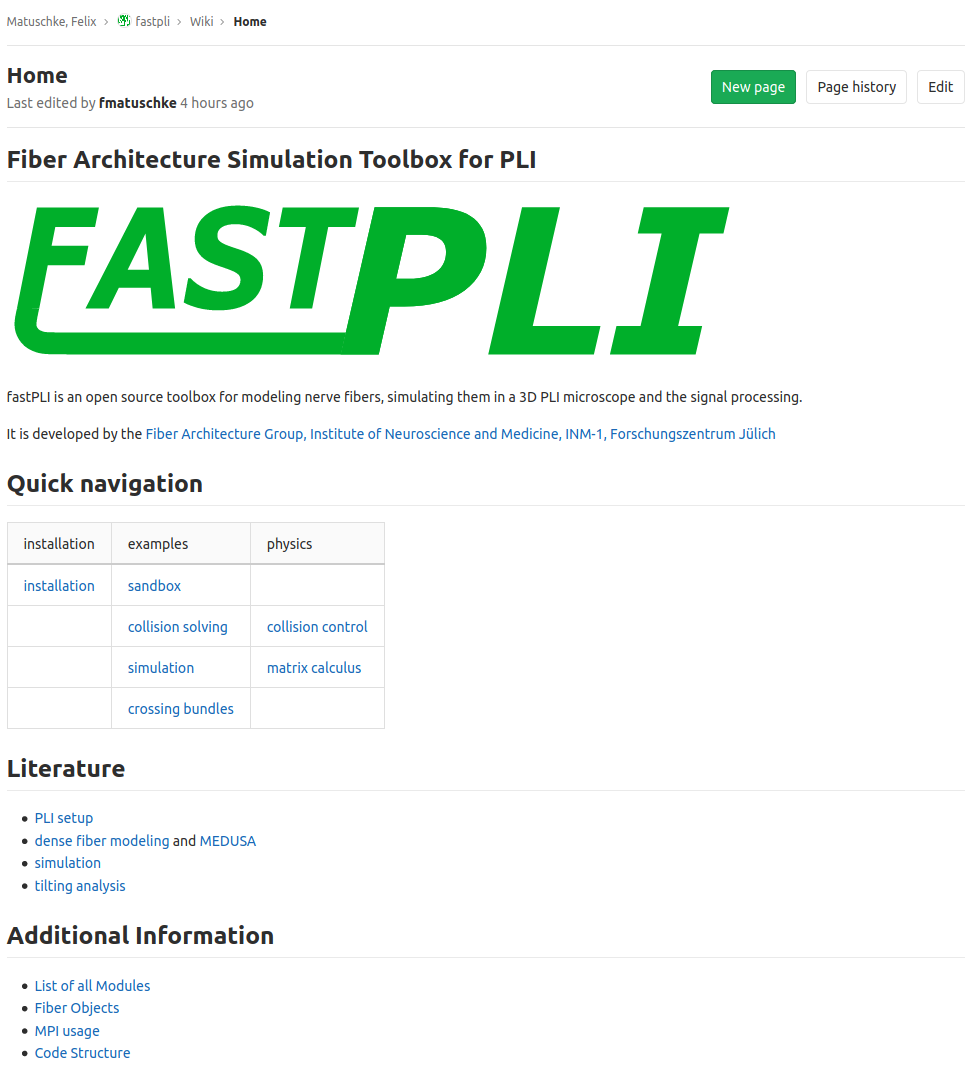
\includegraphics{gfx/fastpli/fastpli_wiki_home.png}}}
	\caption{\dummy{}}
	\label{fig:fastpli_wiki_home}
\end{figure}
% 
\begin{figure}[!t]
    \centering
    \resizebox{\textwidth}{!}{\fbox{
    \begin{tabular}{c|c}
    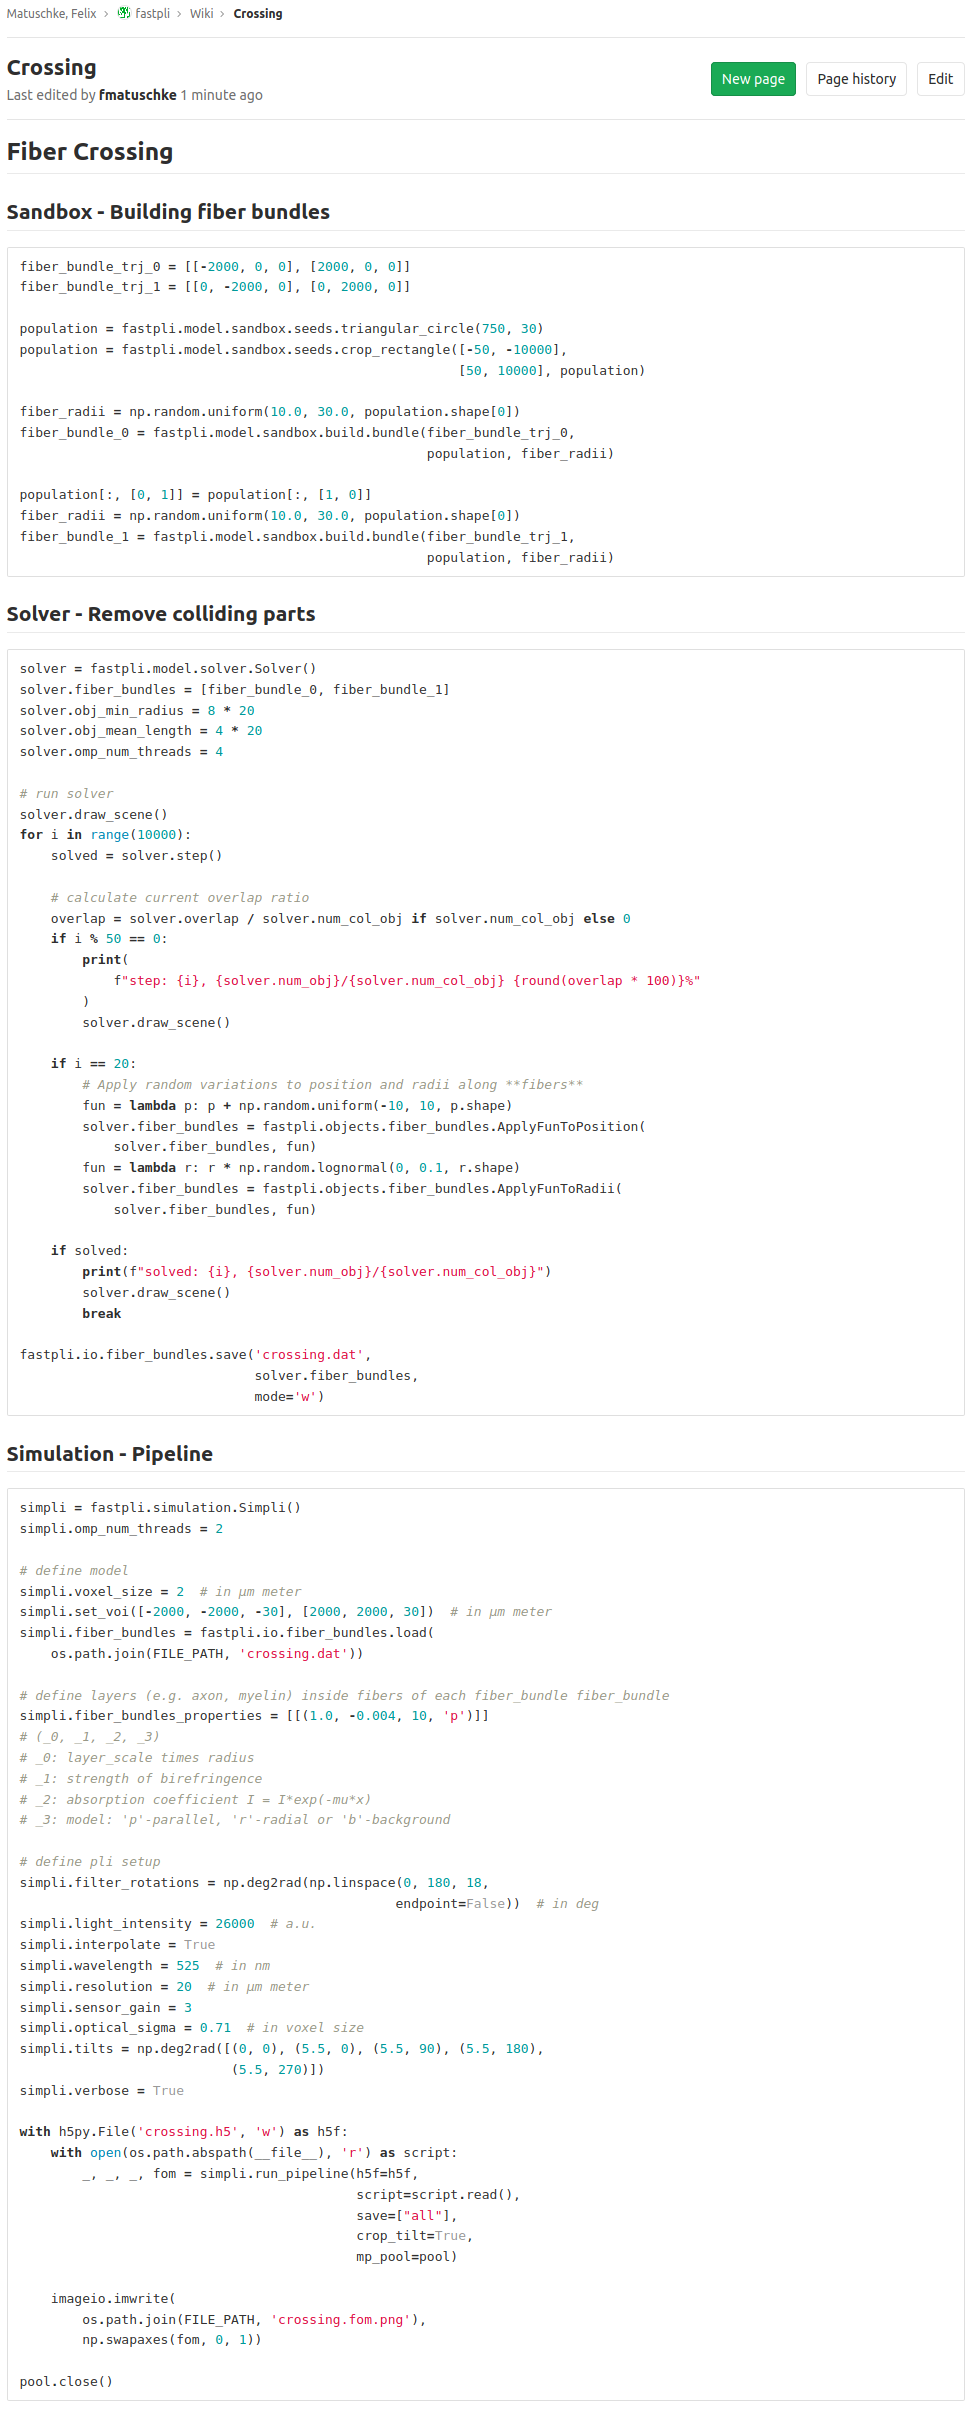
\includegraphics[valign=T]{gfx/fastpli/fastpli_wiki_crossing_left.png} &
 	\includegraphics[valign=T]{gfx/fastpli/fastpli_wiki_crossing_right.png} \\
    \end{tabular}
    }}
	\caption{\dummy{}}
	\label{fig:fastpli_wiki_crossing}
\end{figure}
% 
% 
% A Python packages is a seperated into \code{modules}.
% A Python packages is the overhaul collection of all modules and instructions.
% Models  \begin{quote}
%     A module can contain executable statements as well as function definitions. [\,\dots] Modules can import other modules.
% \end{quote}

% \begin{figure}[!h]
% \begin{lstlisting}[language=python]
% import my-package.my-module
% \end{lstlisting}
% \label{fig:python_test}
% \caption{python test.}
% \end{figure}


%
%\begin{figure}[!t]
%	\centering
%	\resizebox{\textwidth}{!}{
%		\tikzfigure{mindmap}
%	}
%	\label{fig:mindmap}
%	\caption{mindmap.}
%\end{figure}
%
% \begin{figure}
% 	\centering
% 	\resizebox{\textwidth}{!}{
% 	\tikzfigure{uml-example}
% 	}
% \end{figure}
%
% \begin{figure}[!t]
% 	\centering
% 	\resizebox{\textwidth}{!}{
% 		\inputtikz{gfx/fastpli/fastpli_diagram}
% 	}
% 	\label{fig:fastpli_diagram}
% 	\caption{fastpli diagram.}
% \end{figure}
%
% \begin{figure}[!t]
% 	\lstinputlisting[language=python]{code/dummy.py}
% 	\label{fig:python_test}
% 	\caption{python test.}
% \end{figure}
%